\documentclass[12pt]{article}

% --- Packages ---
\usepackage[utf8]{inputenc}
\usepackage{graphicx}
\usepackage{amsmath}
\usepackage{booktabs}
\usepackage{float}
\usepackage{natbib}
\usepackage{geometry}
\usepackage{setspace}
\usepackage{caption}

\geometry{margin=1in}
\setstretch{1.25}

% --- Title Info ---
\title{Comparative Analysis of Diabetes Risk in Pima and NHANES Populations}
\author{Laurentiu-Nicolae Fratila}
\date{\today}

% --- Start Document ---
\begin{document}

\maketitle

\begin{abstract}
This report investigates and compares diabetes-related health indicators in two different populations: the Pima Indian cohort and a sample from the U.S. population based on the NHANES 2017–2018 survey. Statistical analyses were conducted on variables such as glucose levels, BMI, age, and diabetes prevalence.
\end{abstract}

\section{Introduction}
Diabetes is a chronic disease with rising prevalence worldwide. Certain populations, such as the Pima Indians, show particularly high risk. This study compares key health indicators between a dataset of Pima Indian women and a sample of U.S. women from NHANES.

\section{Data and Methods}

\subsection{Pima Indian Diabetes Dataset}
The Pima Indian dataset is a widely used public dataset originally collected by the National Institute of Diabetes and Digestive and Kidney Diseases. It consists of 768 female patients of Pima Indian heritage, all aged 21 or older. Each observation includes numeric variables such as number of pregnancies, plasma glucose concentration, diastolic blood pressure, skinfold thickness, serum insulin, body mass index (BMI), diabetes pedigree function, and age. The outcome variable is a binary indicator of whether the individual has diabetes (1) or not (0), based on diagnostic criteria at the time.

\subsection{NHANES Dataset}
The National Health and Nutrition Examination Survey (NHANES) is a program of the Centers for Disease Control and Prevention (CDC) that collects health-related data on a representative sample of the U.S. population. For this study, we used the 2017–2018 cycle and combined data from four components: demographic information, the diabetes questionnaire, fasting glucose lab values, and body measures. We restricted the sample to adult females aged 21 years and older, to align it with the Pima dataset.

\subsection{Variable Harmonization}
To allow comparison between the two datasets, we selected common variables: age, BMI, fasting plasma glucose, and diabetes status. In NHANES, diabetes status was derived from the self-reported variable \texttt{DIQ010}, with a value of 1 interpreted as a positive diabetes diagnosis. Gender was harmonized by selecting only female participants. Variables were renamed and cleaned to match those in the Pima dataset.

\subsection{Statistical Analysis}
All statistical analyses were performed in R. Descriptive statistics were computed for age, BMI, glucose, and diabetes prevalence in both datasets. We used two-sample t-tests to compare the mean values of continuous variables and a chi-square test to compare proportions of diabetes diagnosis between groups. Logistic regression models were fit separately on each dataset to assess the relationship between age, BMI, and glucose as predictors of diabetes status.

All plots were exported in Encapsulated PostScript (EPS) format to ensure compatibility with LaTeX.


\section{Results}

\subsection{Descriptive Statistics}
Table~\ref{tab:summary-stats} summarizes the average values of age, BMI, and glucose in the two cohorts. On average, the NHANES sample is older but has lower BMI and glucose levels than the Pima Indian sample.

\begin{table}[H]
\centering
\caption{Descriptive statistics for both datasets}
\label{tab:summary-stats}
\begin{tabular}{lccc}
\toprule
\textbf{Variable} & \textbf{Pima (mean)} & \textbf{NHANES (mean)} & \textbf{p-value} \\
\midrule
Age (years)     & 33.24  & 45.70   & $<$0.001 \\
BMI (kg/m$^2$)  & 31.99  & 28.96   & $<$0.001 \\
Glucose (mg/dL) & 120.89 & 111.82  & $<$0.001 \\
\bottomrule
\end{tabular}
\end{table}

\subsection{Visual Comparison of Distributions}

\begin{figure}[H]
\centering
\includegraphics[width=0.8\textwidth]{glucose_histogram.eps}
\caption{Distribution of fasting glucose levels in Pima and NHANES datasets.}
\end{figure}

\begin{figure}[H]
\centering
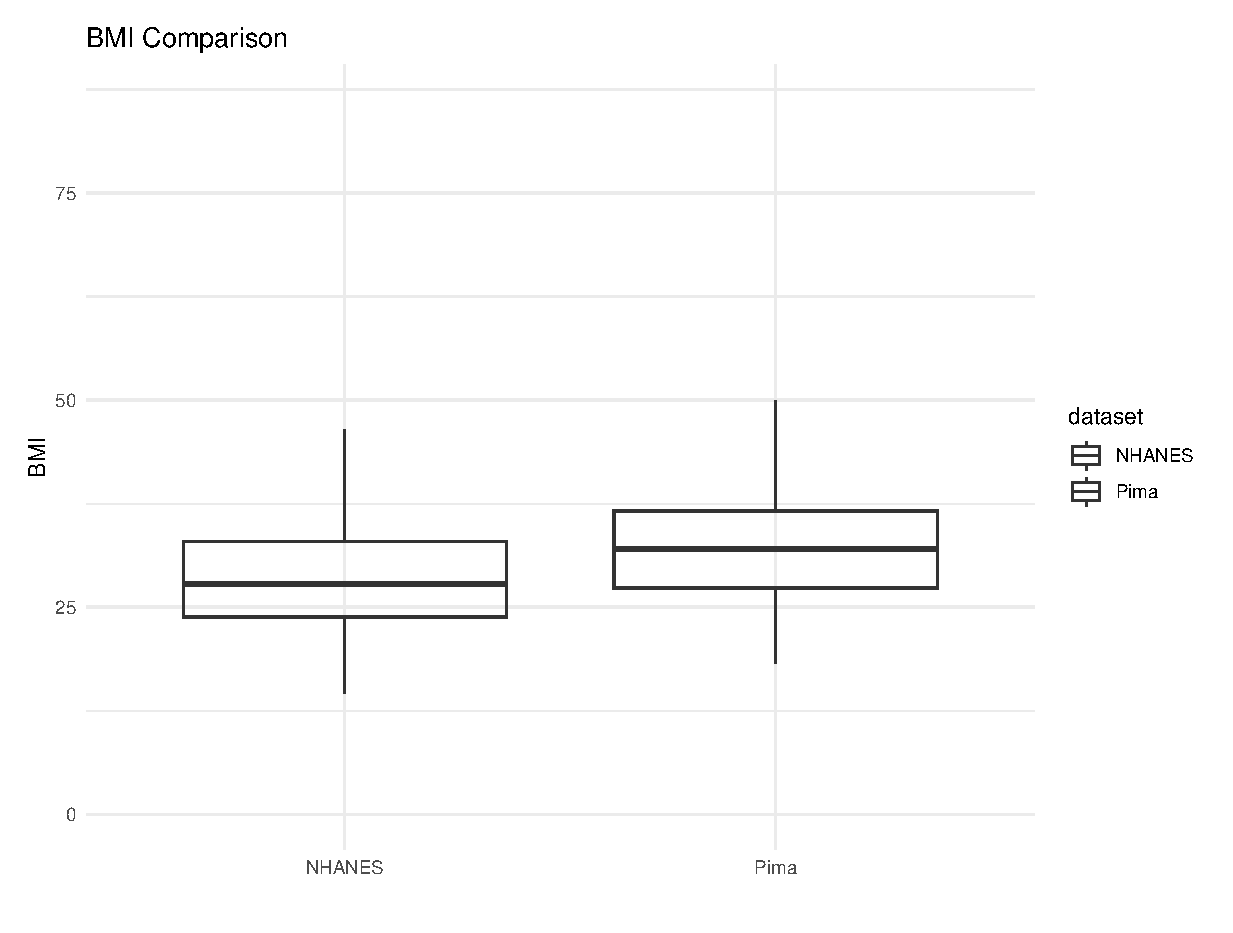
\includegraphics[width=0.8\textwidth]{bmi_boxplot.eps}
\caption{Comparison of BMI between Pima and NHANES cohorts.}
\end{figure}

\begin{figure}[H]
\centering
\includegraphics[width=0.8\textwidth]{diabetes_barplot.eps}
\caption{Diabetes prevalence in Pima vs NHANES groups.}
\end{figure}

\subsection{Inferential Statistics}
Two-sample t-tests confirmed significant differences in age, BMI, and glucose between the groups ($p < 0.001$ for all comparisons). A chi-square test for diabetes prevalence yielded a significant result ($\chi^2 = 167.02$, $df = 1$, $p < 0.001$), suggesting that diabetes rates differ significantly between the populations.

\subsection{Logistic Regression Models}
Separate logistic regression models were fitted on each dataset to predict diabetes status using age, BMI, and glucose as predictors. The results are summarized in Table~\ref{tab:logreg}.

\begin{table}[H]
\centering
\caption{Logistic regression results: coefficients and p-values}
\label{tab:logreg}
\begin{tabular}{lcccc}
\toprule
\textbf{Predictor} & \multicolumn{2}{c}{\textbf{Pima}} & \multicolumn{2}{c}{\textbf{NHANES}} \\
\cmidrule(lr){2-3} \cmidrule(lr){4-5}
& Coef & $p$-value & Coef & $p$-value \\
\midrule
Age       & 0.030 & 7.77e-05 & 0.058 & $<$0.001 \\
BMI       & 0.082 & $<$0.001 & 0.054 & $<$0.001 \\
Glucose   & 0.033 & $<$0.001 & 0.041 & $<$0.001 \\
\bottomrule
\end{tabular}
\end{table}


\section{Discussion and Conclusion}

This study compared diabetes-related indicators between the Pima Indian cohort and a subset of the general U.S. population from the NHANES 2017–2018 survey. The Pima dataset, which includes only adult women of Pima Indian heritage, is known for a high prevalence of type 2 diabetes. The NHANES sample was filtered to include only adult women aged 21 and older, to match the characteristics of the Pima group as closely as possible.

Our findings reveal statistically significant differences in all key health indicators. The NHANES participants were, on average, older but had lower mean BMI and glucose levels. Diabetes prevalence was significantly higher in the Pima group compared to NHANES. These results are consistent with previous literature that identifies Native American populations as having elevated diabetes risk due to genetic, socioeconomic, and environmental factors.

Logistic regression models showed that age, BMI, and glucose levels were all significant predictors of diabetes status in both datasets. Glucose had the strongest predictive value, followed by BMI. The higher coefficient for age in the NHANES model likely reflects the wider age distribution and older mean age in that population.

This study highlights the importance of population-specific risk profiles in diabetes screening and prevention strategies. Although models trained on one population may be generalizable, they should be validated carefully before clinical application across diverse groups.

\textbf{Limitations:} The NHANES diabetes status is based on self-reported diagnosis, which may lead to underestimation. The Pima dataset is limited in scope and lacks some variables that NHANES includes, such as HbA1c levels. Furthermore, the study does not account for socioeconomic or lifestyle differences between the populations.

\textbf{Conclusion:} The Pima Indian cohort displays significantly higher diabetes prevalence and risk factor levels compared to a nationally representative female sample. This reinforces the need for targeted interventions and supports the broader use of biostatistical modeling for population health management.

\section*{References}

\begin{enumerate}
    \item Centers for Disease Control and Prevention. National Health and Nutrition Examination Survey (NHANES) 2017–2018. \textit{Available at:} \texttt{https://www.cdc.gov/nchs/nhanes/index.htm}
    
    \item National Center for Health Statistics. NHANES 2017–2018 Datasets. \textit{Available at:} \texttt{https://wwwn.cdc.gov/nchs/nhanes/continuousnhanes/default.aspx?BeginYear=2017}
    
    \item UCI ML Repository. Pima Indians Diabetes Database. \textit{Available at:} \texttt{https://www.kaggle.com/datasets/uciml/pima-indians-diabetes-database}
    
    \item American Diabetes Association. Standards of Medical Care in Diabetes—2024. \textit{Diabetes Care}. 2024;47(Suppl 1):S1–S154. \textit{Available at:} \texttt{https://diabetesjournals.org/care/article/47/Supplement\_1/S1/152058}
    
    \item Wild S, Roglic G, Green A, Sicree R, King H. Global prevalence of diabetes: Estimates for 2000 and projections for 2030. \textit{Diabetes Care}. 2004;27(5):1047–1053.
\end{enumerate}


\end{document}
